\section{Design API Rest}
\subsection{Description}

\begin{flushleft}
Afin d'interagir entre l'application et la base de données, des requêtes sont envoyées via l'API Rest permettant cette communication. C'est pourquoi certains services ont été ajoutés à la base commune de l'API.
Pour les mêmes raisons que la partie commune, le \textbf{token} de connexion est repris à chaque fois
\end{flushleft}

\begin{flushleft}
Pour qu'un client puisse voir la liste de ses factures, une requête \textbf{GET} doit être envoyée. Dans cette requête, un paramètre \emph{id-facture} est nécessaire pour voir une facture en particulier. Si ce paramètre vaut \textbf{NULL}, toutes les factures sont affichées.
Cette requête renvoie donc un objet \emph{Facture} comprenant les mêmes éléments cités précédemment.
\end{flushleft}

\begin{flushleft}
Un client peut modifier l'acompte proposé par l'application. C'est pourquoi, une requête \textbf{PUT} peut être envoyée contenant un paramètre \emph{account} spécifiant la nouvelle valeur de l'acompte.
De la même manière, les informations de paiement et informations bancaires peuvent être modifiées à l'aide du même type de requête.
Il faut cependant noter que le paramètre \emph{id-facture} ne peut plus être \textbf{NULL} sous peine de générer une erreur.
\end{flushleft}

\newpage
\begin{figure}[h]
\subsection{Schéma}
\centering
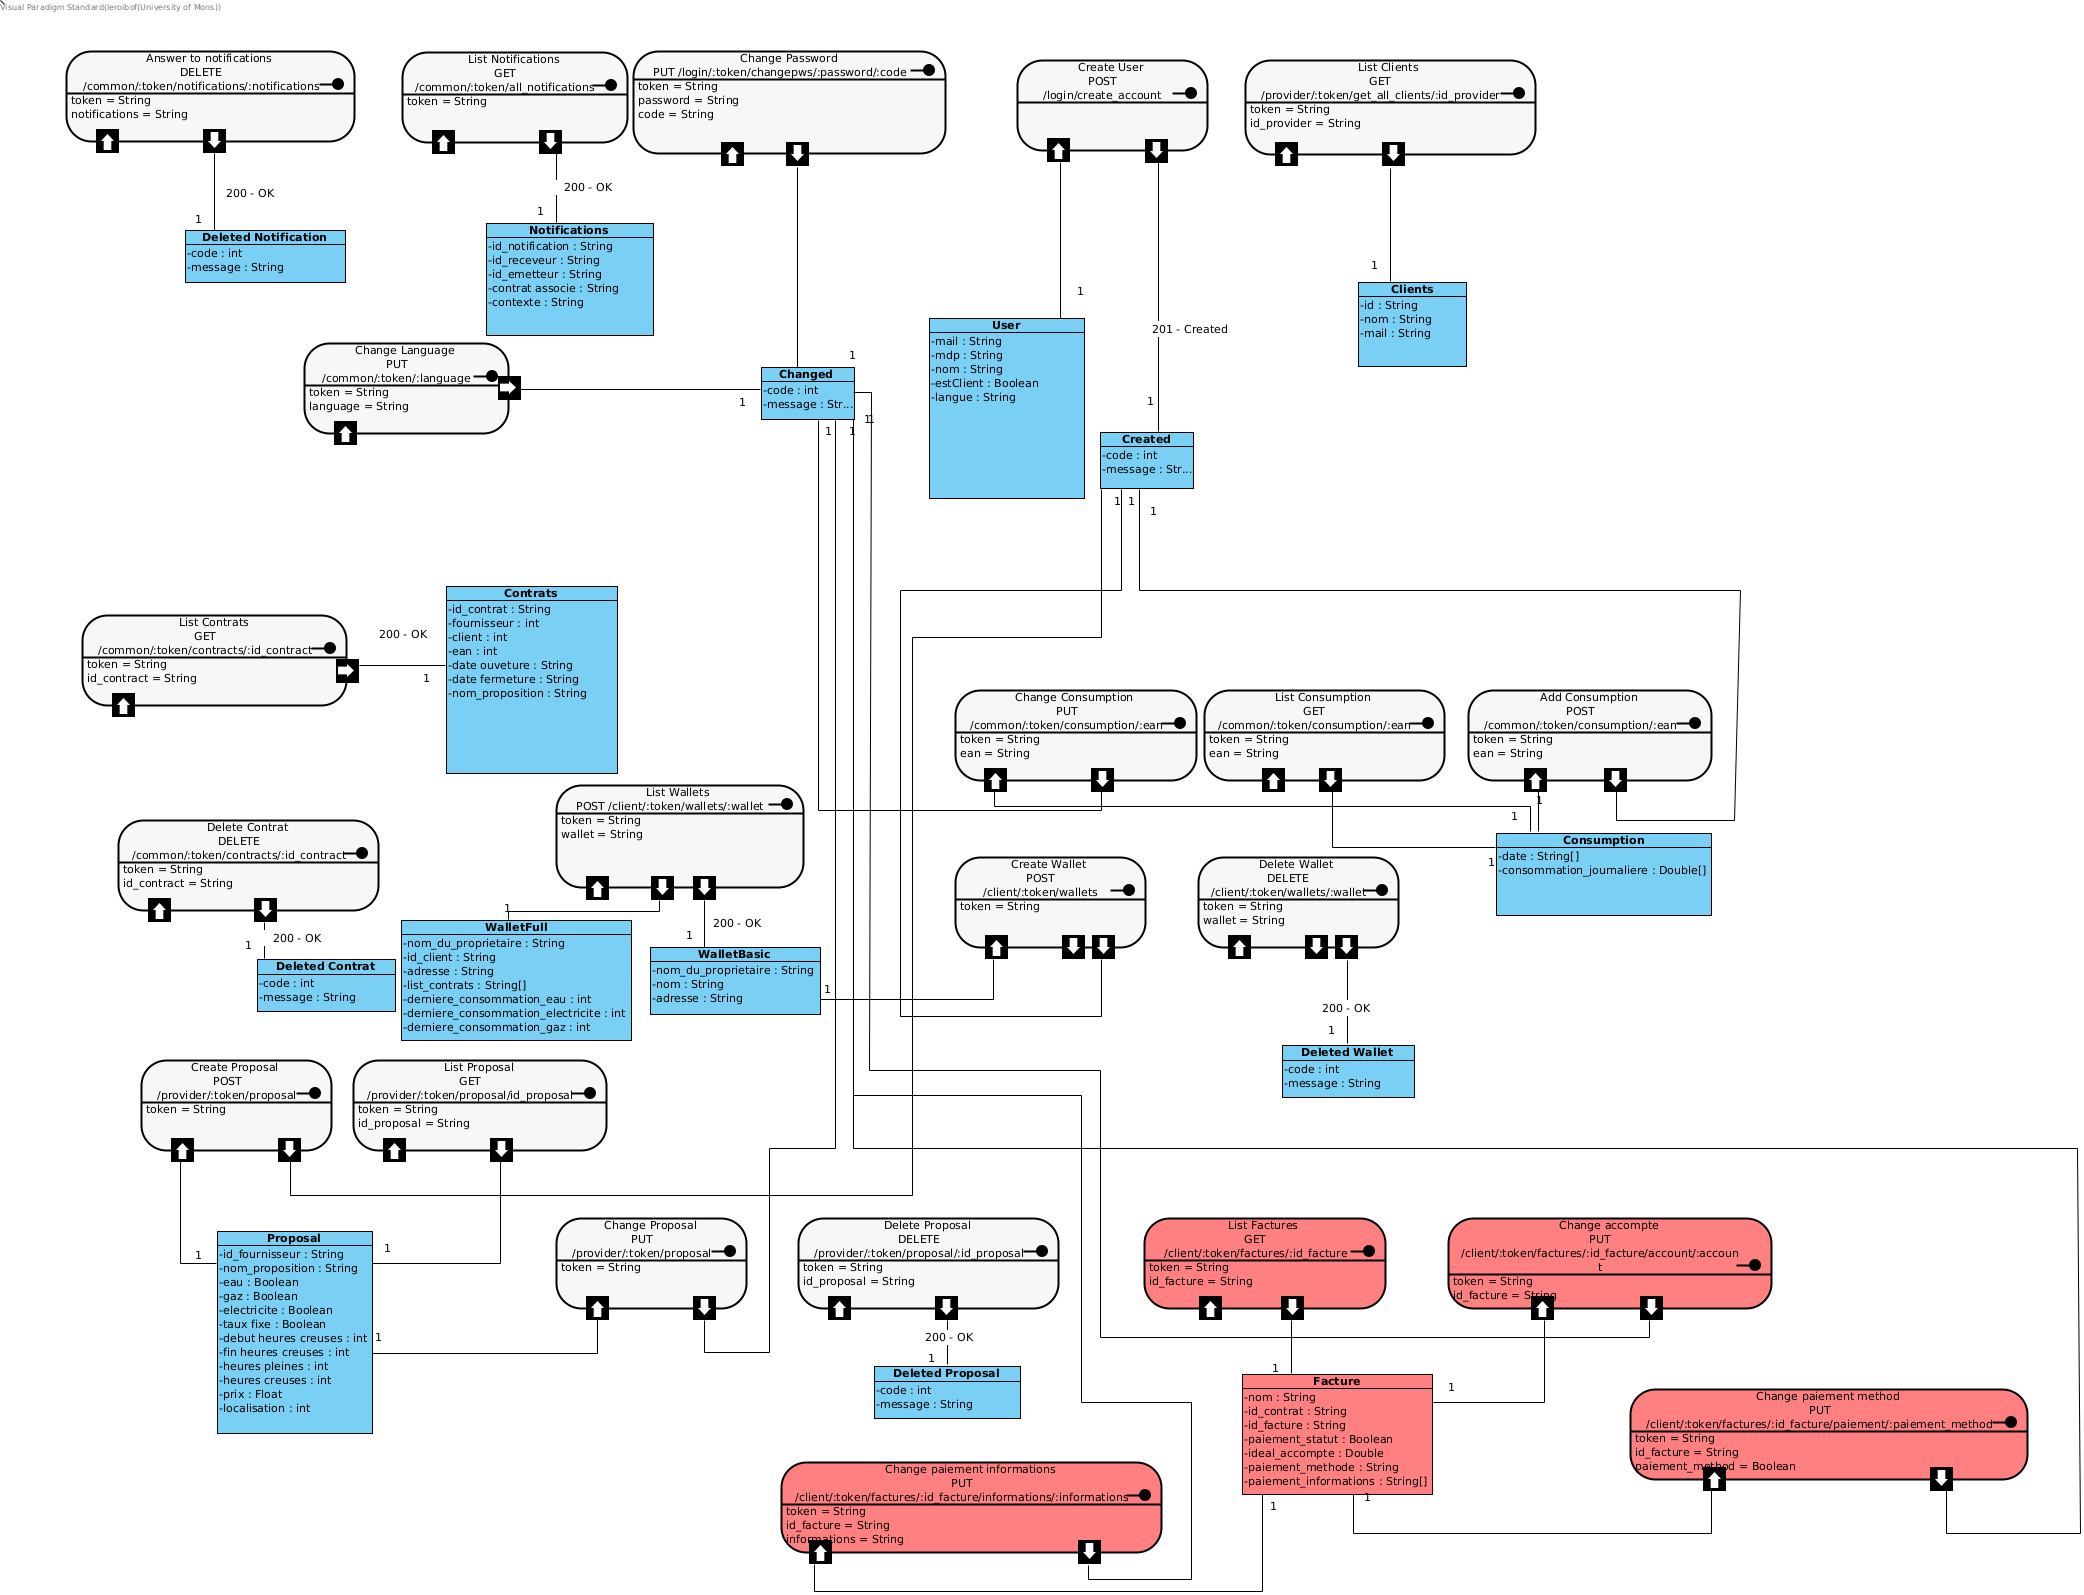
\includegraphics[width = 1.2\textwidth]{extension-maxime/apirest/img/apirest-extension.png}
\end{figure}
